\section{Fundamentalsatz der Algebra}

\begin{remark}
	\proplbl{2_4_1}
	Wir werden die folgende Eigenschaften der Körper $\mathbb R$ und $\mathbb C$ benutzen: \begin{remarkenum}[]
		\item \proplbl{2_4_1_1} $\mathbb C=\mathbb R(i)$ mit $i^2 = -1$,
		\item \proplbl{2_4_1_2} $a\in\mathbb R$, $a > 0$ $\Rightarrow$ $\sqrt a\in\mathbb R$
		\item \proplbl{2_4_1_3} $f\in\mathbb R[X]$, $\deg(f)$ ungerade $\Rightarrow$ $f$ hat Nullstelle in $\mathbb R$
	\end{remarkenum}
\end{remark}

\begin{lemma}
	\proplbl{2_4_2}
	Sei $K\subseteq L\subseteq \bar K$ eine Erweiterung von $K$. Dann gibt es eine kleinste Erweiterung $K\subseteq \hat L\subseteq \bar K$ mit $\hat L\mid K$ normal.
	
	Ist $L\mid K$ endlich, so ist auch $\hat L\mid K$ endlich.
	
	Ist $L\mid K$ separabel, so auch $\hat L\mid K$.
\end{lemma}

\begin{proof}
	klar, da $\hat L = K \big( \cup_{\sigma\in\Aut(\bar K\mid K)} L^\sigma\big)$. Für $\tau\in\Aut(\bar K, K)$ ist dann $\hat L^\tau = K\big( \cup_{\sigma} L^{\sigma\tau}\big) = K\big( \cup_\sigma L^\sigma\big) = \hat L$.
	\begin{itemize}[topsep=-6pt]
		\item endlich: Ist $L= K(\alpha_1,\dots,\alpha_n)$, so ist $\hat L$ der Zerfällungskörper von \begin{align*}
			f := \prod_{i=1}^n \MinPol(\alpha_i\mid K)
		\end{align*}
		\item separabel: $L\mid K$ separabel $\Rightarrow$ $L^\sigma\mid K$ separabel $\xRightarrow{\propref{1_7_6}}$ $K\big(\cup_\sigma L^\sigma\big) \mid K$ separabel
	\end{itemize}
\end{proof}

\begin{definition}
	$\hat L$ ist die \begriff{normale Hülle} von $L\mid K$.
\end{definition}

\begin{theorem}
	\proplbl{2_4_4}
	$\mathbb C = \bar{\mathbb C}$.
\end{theorem}

\begin{proof}
	Unter Benutzung \cref{2_4_1_1,2_4_1_2,2_4_1_3}. \begin{enumerate}[label={Beh. \arabic*:},left=0pt,labelwidth=7em,topsep=-6pt,align=left,ref={Beh.~\arabic*}]
		\item \proplbl{2_4_4_1} Jedes $z=a+b\imath\in\mathbb C$ hat eine Quadratwurzel in $\mathbb C$ ($a$, $b\in\mathbb R$)
		\begin{proof}
			$z=a+b\imath = (x + y\imath)^2 = x^2 + y^2 + 2xy\imath $ ($x$, $y\in\mathbb R$) \begin{itemize}[topsep=-6pt,label={$\Rightarrow$}]
				\item $a = x^2 - y^2$, $b = 2xy$
				\item $a = x^2 - \Big(\frac b{2x}\Big)^2$
				\item $x^4 - ax^2 - \frac14 b^2 = 0$
			\end{itemize}
			\medskip		
			$w^2 - aw - \frac14 b^2 = 0$ hat die Lösung \begin{align*}
				w = \frac{a \pm \sqrt{a^2 + b^2}}{2} \in\mathbb R,
			\end{align*}
			nach \propref{2_4_1_2}.
			
			Wähle $w > 0$ $\xRightarrow{\propref{2_4_1_2}}$ ex. $x\in\mathbb R$ mit $x^4 - ax^2 - \frac14 b^2 = 0$
		\end{proof}
	
		\item \proplbl{2_4_4_2} $\mathbb C$ hat keine Erweiterung vom Grad 2.
		
		\begin{proof}
			$L = \mathbb C(\alpha)$, $[L:\mathbb C] = 2$ \begin{itemize}[topsep=-6pt,widest={$\xRightarrow{\text{\ref{2_4_4_1}}}$},leftmargin=*]
				\item[$\xRightarrow{\text{Ü20}}$] o.E. $\alpha^2\in\mathbb C$
				\item[$\xRightarrow{\text{\ref{2_4_4_1}}}$] $\alpha\in \mathbb C$.
			\end{itemize}
		\end{proof}
	
		\item \proplbl{2_4_4_3} $\mathbb R$ hat keine Erweiterung ungeraden Grades.
		
		\begin{proof}
			$[L\mid\mathbb R] = n$ ungerade \begin{itemize}[topsep=-6pt,label={$\Rightarrow$},widest={$\xRightarrow{\propref{1_9_5}}$},leftmargin=*]
				\item[$\xRightarrow{\propref{1_9_5}}$] $L=\mathbb R(\alpha)$ für ein $\alpha$
				\item $f:=\MinPol(\alpha\mid\mathbb R)$ hat Grad $\deg(f) = \deg(\alpha\mid \mathbb R) = [\mathbb R(\alpha):\mathbb R] = n$ ungerade
			\end{itemize}
			\begin{align*}
				\hspace*{-3em}\left.\begin{array}{@{}l}
					f\;\text{ist irreduzibel} \\
					f\;\text{hat Nullstelle in $\mathbb R$ nach \propref{2_4_1_3}}
				\end{array}\right\rbrace \quad\Rightarrow\quad \deg(f) = 1\quad\Rightarrow\quad L =\mathbb R
			\end{align*}
		\end{proof}
	
		\item $\mathbb C$ hat keine echten endlichen Erweiterungen.
		
		\begin{proof}
			Sei $L\mid\mathbb C$ endlich. Sei $M$ die normale Hülle $L\mid\mathbb R$, $G:=\Gal(M\mid \mathbb R)$, $H:= \Gal(M\mid \mathbb C)$, $S := \Syl_2(G)$, $K=M^S$
					
			\begin{minipage}{0.6\linewidth}
			\begin{itemize}[topsep=-6pt,label={$\Rightarrow$},widest={$\xRightarrow{\text{GEO~I.7.9}}$},leftmargin=*]
				\item $[K:\mathbb R] = (G:S)$ ungerade
				\item[$\xRightarrow{\text{\ref{2_4_4_3}}}$] $K=\mathbb R$, $G=S$ ist 2-Gruppe.
			\end{itemize}
			\medskip
			Angenommen $\# G = 2^k$, $k\ge 2$\begin{itemize}[topsep=-6pt,label={$\Rightarrow$},widest={$\xRightarrow{\text{GEO~I.7.9}}$},leftmargin=*]
				\item[$\xRightarrow{\text{GEO~I.7.9}}$] ex. $U\le H$ mit $(H:U) = 2$
				\item $[M^U:\underbrace{M^H}_{\mathclap{=\mathbb C}}] = (H:U)$ \Lightning\ zu \ref{2_4_4_2}
			\end{itemize}
			\bigskip
			\end{minipage}%
			\hfill%
			\begin{minipage}{0.35\linewidth}
				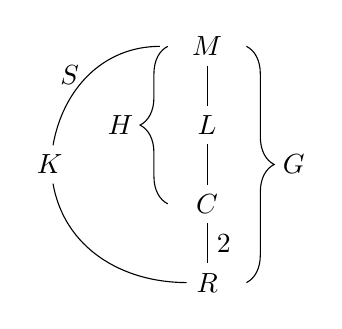
\begin{tikzpicture}
				\node at (0,0) (M) {$M$};
				\node at (0,-1) (L) {$L$};
				\node at (0,-2) (C) {$\mathbb{C}$};
				\node at (0,-3) (R) {$\mathbb{R}$};
				\node at (-2,-1.5) (K) {$K$};
				
				\draw (M) -- (L);
				\draw (L) -- (C);
				\draw (C) to node [right] {2} (R);
				\draw (K) to [out=80,in=180] node [left] {$S$} (-0.6,0);
				\draw (K) to [out=280,in=180] (R);
				
				\draw [decorate,decoration={brace,amplitude=10pt},xshift=-0.5cm,yshift=0pt]
				(1,0) -- (1,-3) node [black,midway, xshift=0.6cm]{$G$};
				\draw [decorate,decoration={brace,amplitude=10pt,mirror},xshift=-0.5cm,yshift=0pt]
				(0,0) -- (0,-2) node [black,midway, xshift=-0.6cm]{$H$};
				\end{tikzpicture}
			\end{minipage}
			Somit ist $\# G = 2$, $\# H=1$, $M=\mathbb C$ $\Rightarrow$ $L=\mathbb C$.
		\end{proof}
	\end{enumerate}
	Ein Körper ist genau dann abgeschlossen, wenn er keine echte algebraische Erweiterung besitzt.
\end{proof}

\begin{remark}
	\proplbl{2_4_5}
	Körper, die eine Anordnung $<$ besitzen und \cref{2_4_1_2,2_4_1_3} erfüllen, nennt man reell abgeschlossen.
\end{remark}

\begin{example}
	$\mathbb R\cap \bar{\mathbb Q}$ ist reell abgeschlossen.
\end{example}